\begin{figure}[t]
  \centering\usetikzlibrary{shapes.arrows}
  \definecolor{tile0}{HTML}{DABDE4}
  \definecolor{tile1}{HTML}{B8DBF4}
  \definecolor{tile2}{HTML}{B5EDCD}
  \definecolor{tile3}{HTML}{FBEBA7}
  \definecolor{tile4}{HTML}{F9C1BB}
  \definecolor{tile5}{rgb}{1, 1, 1}

  \tikzstyle{array_element}=[rectangle,
                             minimum height=1.0cm, 
                             minimum width=1.0cm, 
                             minimum size=1.0cm,
                             draw=black,
                             rounded corners=2.5 ]

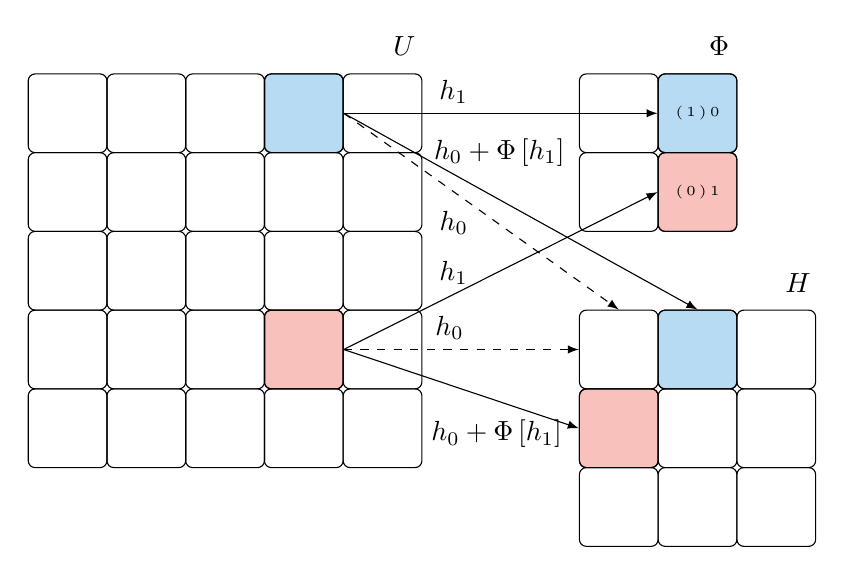
\begin{tikzpicture}
    \node at (3.0cm, 4cm) (UC1) [array_element, fill=tile1] {};
    \node at (3.0cm, 1.0cm) (UC2) [array_element, fill=tile4] {};
    \foreach \la in {0,...,4} {
        \foreach \lb in {0,...,4} {
            \node at (1.0cm * \la, 1.0cm * \lb) () [array_element] {};
        }
    }

    \node at(0.275cm + 4cm, 4.85cm) (U) [] {$U$};
    \node at(0.275cm + 7cm + 1cm, 4.85cm) (U) [] {$\Phi$};
    \node at(0.275cm + 7cm + 2cm, 1.85cm) (U) [] {$H$};

    \node at (8cm, 1.0cm) (HC1) [array_element, fill=tile1] {};
    \node at (7cm, 0cm) (HC2) [array_element, fill=tile4] {};
    
    \foreach \la in {0,...,2} {
        \foreach \lb in {0,...,2} {
            \node at (1.0cm * \la + 7cm, 1.0cm * \lb - 1.0cm) (H\la\lb) [array_element] {};
        }
    }
    
    \node at (8cm, 4cm) (PhiC1) [array_element, fill=tile1] {\tiny $\begin{pmatrix}1 \\ 0\end{pmatrix}$};
    \node at (8cm, 3cm) (PhiC2) [array_element, fill=tile4] {\tiny $\begin{pmatrix}0 \\ 1\end{pmatrix}$};
    \foreach \la in {0,...,1} {
        \foreach \lb in {0,...,1} {
            \node at (1.0cm * \la + 7cm, 1.0cm * \lb + 3cm) () [array_element] {};
        }
    }    
    
    \draw[-latex] (UC1.east) -- (PhiC1.west) node[pos=0.35, above] {$h_1$};
    \draw[-latex] (UC2.east) -- (PhiC2.west) node[pos=0.35, above] {$h_1$};
    
    \draw[-latex] (UC1.east) -- (HC1.north) node[pos=0.2, label=right:{$h_0 + \Phi\left[h_1\right]$}] {};
    \draw[-latex] (UC2.east) -- (HC2.west) node[pos=0.65, label=below:{$h_0 + \Phi\left[h_1\right]$}] {};
    
    \draw[dashed, -latex] (UC1.east) -- (H02.north) node[pos=0.4, label=below:{$h_0$}] {};
    \draw[dashed, -latex] (UC2.east) -- (H02.west) node[pos=0.45, above] {$h_0$};
  \end{tikzpicture}
  \caption{De perfecte spatiale hashfunctie $\mathit{h}\left(\mathbf{p}\right)$.}
  \label{fig:hs-spatiale-hashfunctie}
\end{figure}
